%----------------------------------------------------------------------------------------
%	PACKAGES AND DOCUMENT CONFIGURATIONS
%----------------------------------------------------------------------------------------
\documentclass[a4paper,11pt]{article}
\usepackage{amsmath} % Required for some math elements
\usepackage{hyperref} 
\usepackage{xcolor}
\usepackage{lipsum} 
\usepackage{cite}
\usepackage{graphicx} % Required for the inclusion of images
\usepackage{algorithmic}
\usepackage{array}
\usepackage{bookmark}
\usepackage{listings}
\usepackage{mcode}
\usepackage{amssymb}
\usepackage{enumitem}
\usepackage[margin=32mm,]{geometry}
\usepackage[caption=false, font=footnotesize]{subfig}

\newlist{steps}{enumerate}{1}
\setlist[steps, 1]{label = Step \arabic*:}

\hypersetup{ %color attributes of citation, link, etc.
    colorlinks=true,
    linkcolor=blue,
    filecolor=gray,      
    urlcolor=blue,
    citecolor=blue,
}

\newcommand{\matlab}{\textsc{Matlab }} %very important and totally necessary addition

\newcommand\Item[1][]{%
  \ifx\relax#1\relax  \item \else \item[#1] \fi
  \abovedisplayskip=0pt\abovedisplayshortskip=0pt~\vspace*{-\baselineskip}}
  %----------------------------------------------------------------------------------------
%	DOCUMENT INFORMATION
%----------------------------------------------------------------------------------------
 
\title{ECEN315 LABORATORY REPORT ONE}
\author{Daniel Eisen : 300447549}
\date{\today}

\begin{document}
\maketitle
\section{Introduction}
This project has the goal of creating a system for controlling a pendulum arm driven by a propeller. This necessitates the modelling of system, breaking it sub-blocks/sub-systems and evaluating these models. The work outlined in this report

\section{Background}
In this section you should give a brief background, e.g. control theory and motors.
\newpage
\section{Methodology and Results}
In this section you will explain how to solve the problem, that is, how you performed the project. At this early stage you need to be both clear about what you did and why you did it. You will also explain how you evaluated your solution once you have built it. The method of evaluation will be specific to the tasks. 
\subsection{DC Motor and Propeller}
\begin{figure}[h]
        \centering
        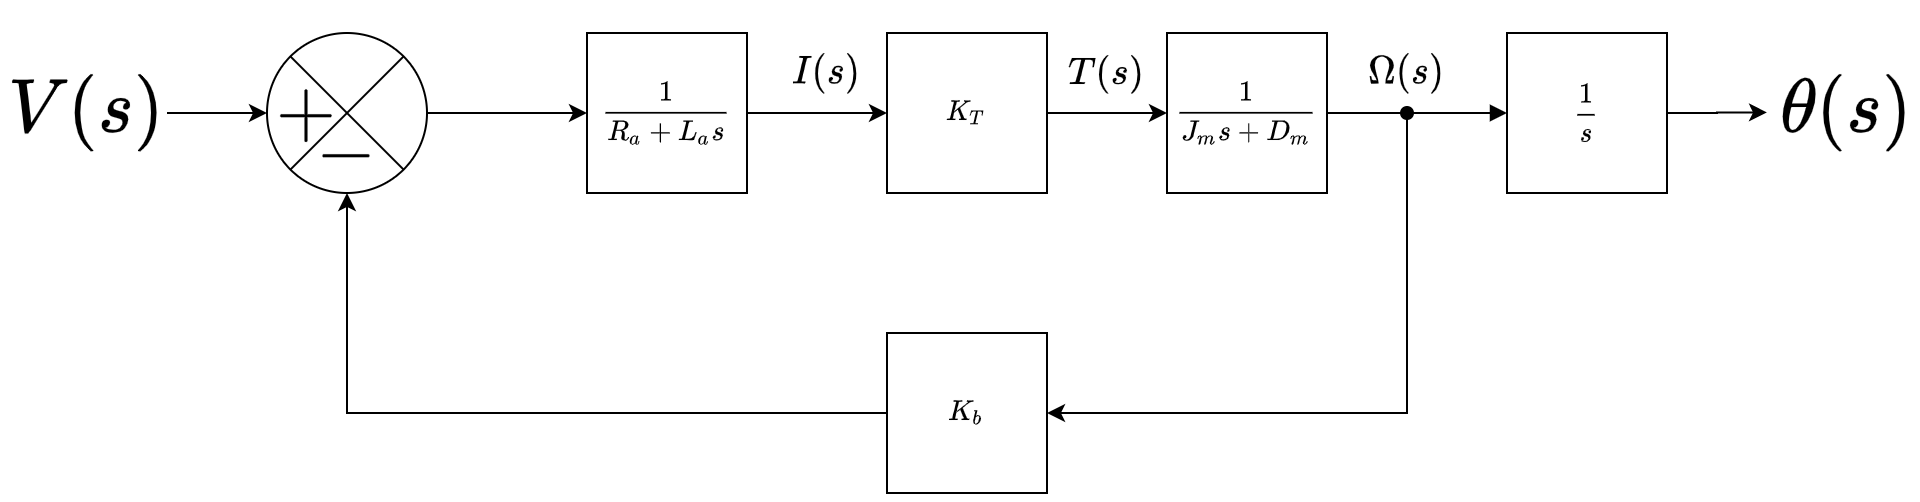
\includegraphics[width=0.75\textwidth]{inc/motor_diagram.png}
        \caption{Block Diagram of DC Motor+Propeller System}
        \label{}
\end{figure}

\begin{align*}
        \frac{\Omega(s)}{V(s)} &= \frac{\frac{K_t}{(R_a+L_{a}s)(D_m+J_{m}s)}}{1+\frac{K_tK_b}{(R_a+L_{a}s)(D_m+J_{m}s)}} \\
                               &= \frac{K_t}{(R_a + L_{a}s)(D_m+J_{m}s) + K_tK_b} \\
                               &= \frac{K_t}{L_aJ_{m}s^{2} + (R_{a}J_{m} + L_aD_{m})s + R_{a}D_{m} + K_tK_b } \\
                               &= \frac{\frac{K_t}{L_aJ_m}}{s^2 + \frac{R_{a}J_{m} + L_{a}D_{m}}{L_{a}J_{a}}s + \frac{R_aD_m + K_tK_b}{L_aJ_m}}
\end{align*}

\begin{figure}[h]
        \centering
        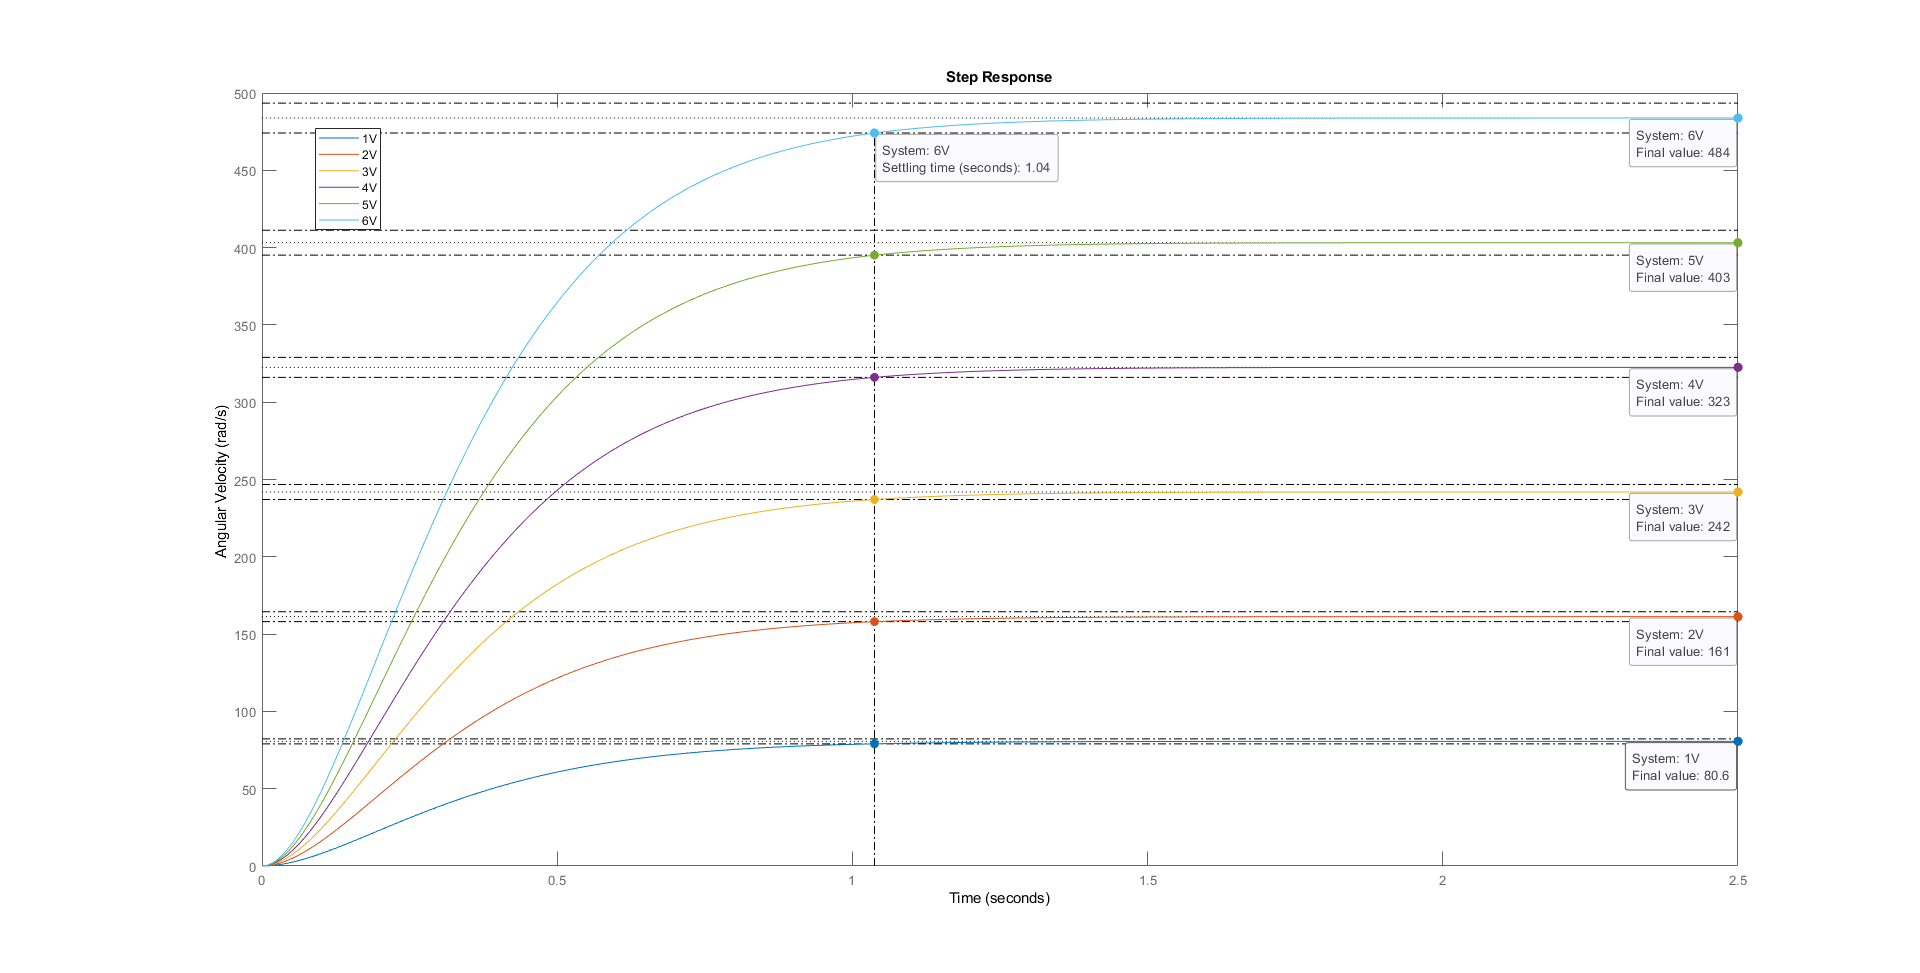
\includegraphics[width=\textwidth]{inc/motor_steps.png}
        \caption{Step response}
        \label{}
\end{figure}
\begin{center}
        \begin{verbatim}
                Steady state gain for V = 1: 80.631551
                Steady state gain for V = 2: 80.631551
                Steady state gain for V = 3: 80.631551
                Steady state gain for V = 4: 80.631551
                Steady state gain for V = 5: 80.631551
                Steady state gain for V = 6: 80.631551
        \end{verbatim}
\end{center}

\newpage
\subsection{Pendulum}
For the driven pendulum, the torque applied to the pendulum must balance with the existing torques, ie from gravity, damping and the arms moment of inertia.
Before the DE is derived, I needed to approximate the torque applied via gravity:
$$\tau_{gravity} = mgd{\cdot}sin(\theta) = mgd{\cdot}\theta$$
This approximation works for small angles, but quickly diverges in accuracy for $\theta \ge \pi/8 \rightarrow \pi/4$ \\

\begin{center}
        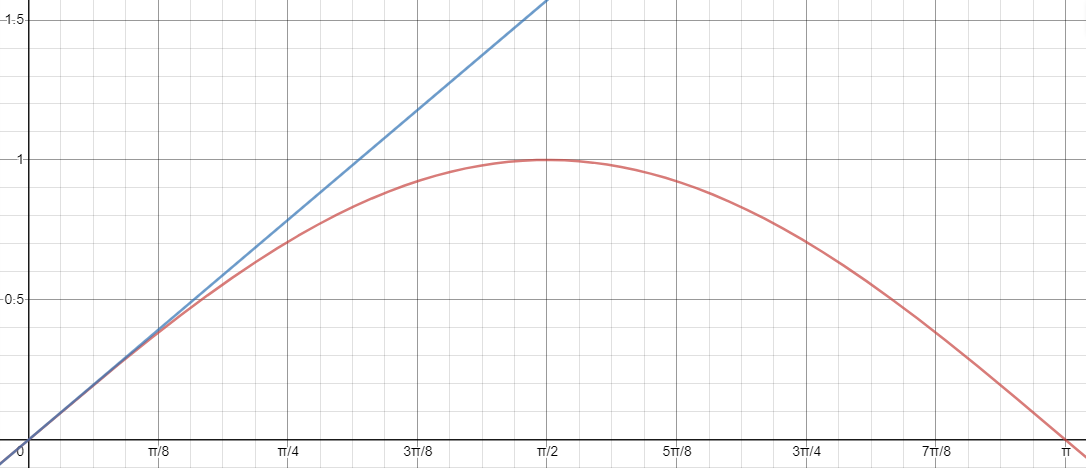
\includegraphics[width=0.45\textwidth]{inc/sintheta.png}
\end{center}
\subsubsection{Differential Equation and Transfer Function}
\begin{align*}
\tau(t) &= J_{p}\frac{d^{2}\Theta}{dt^{2}} + c\frac{d\Theta}{dt} + mgd\Theta \\
T(s) &= J_{p}s^{2}\Theta(s) + cs\Theta(s) + mgd\Theta(s) \\
\frac{\Theta(s)}{T(s)} &= \frac{1}{J_{p}s^{2} + cs + mgd} \\
&=  \frac{\frac{1}{J_{p}}}{s^{2} + \frac{c}{J_{p}}s + \frac{mgd}{J_{p}}}
\end{align*}

\subsubsection{Calculating Damping and Inertia}

\begin{figure}[h]
        \centering
        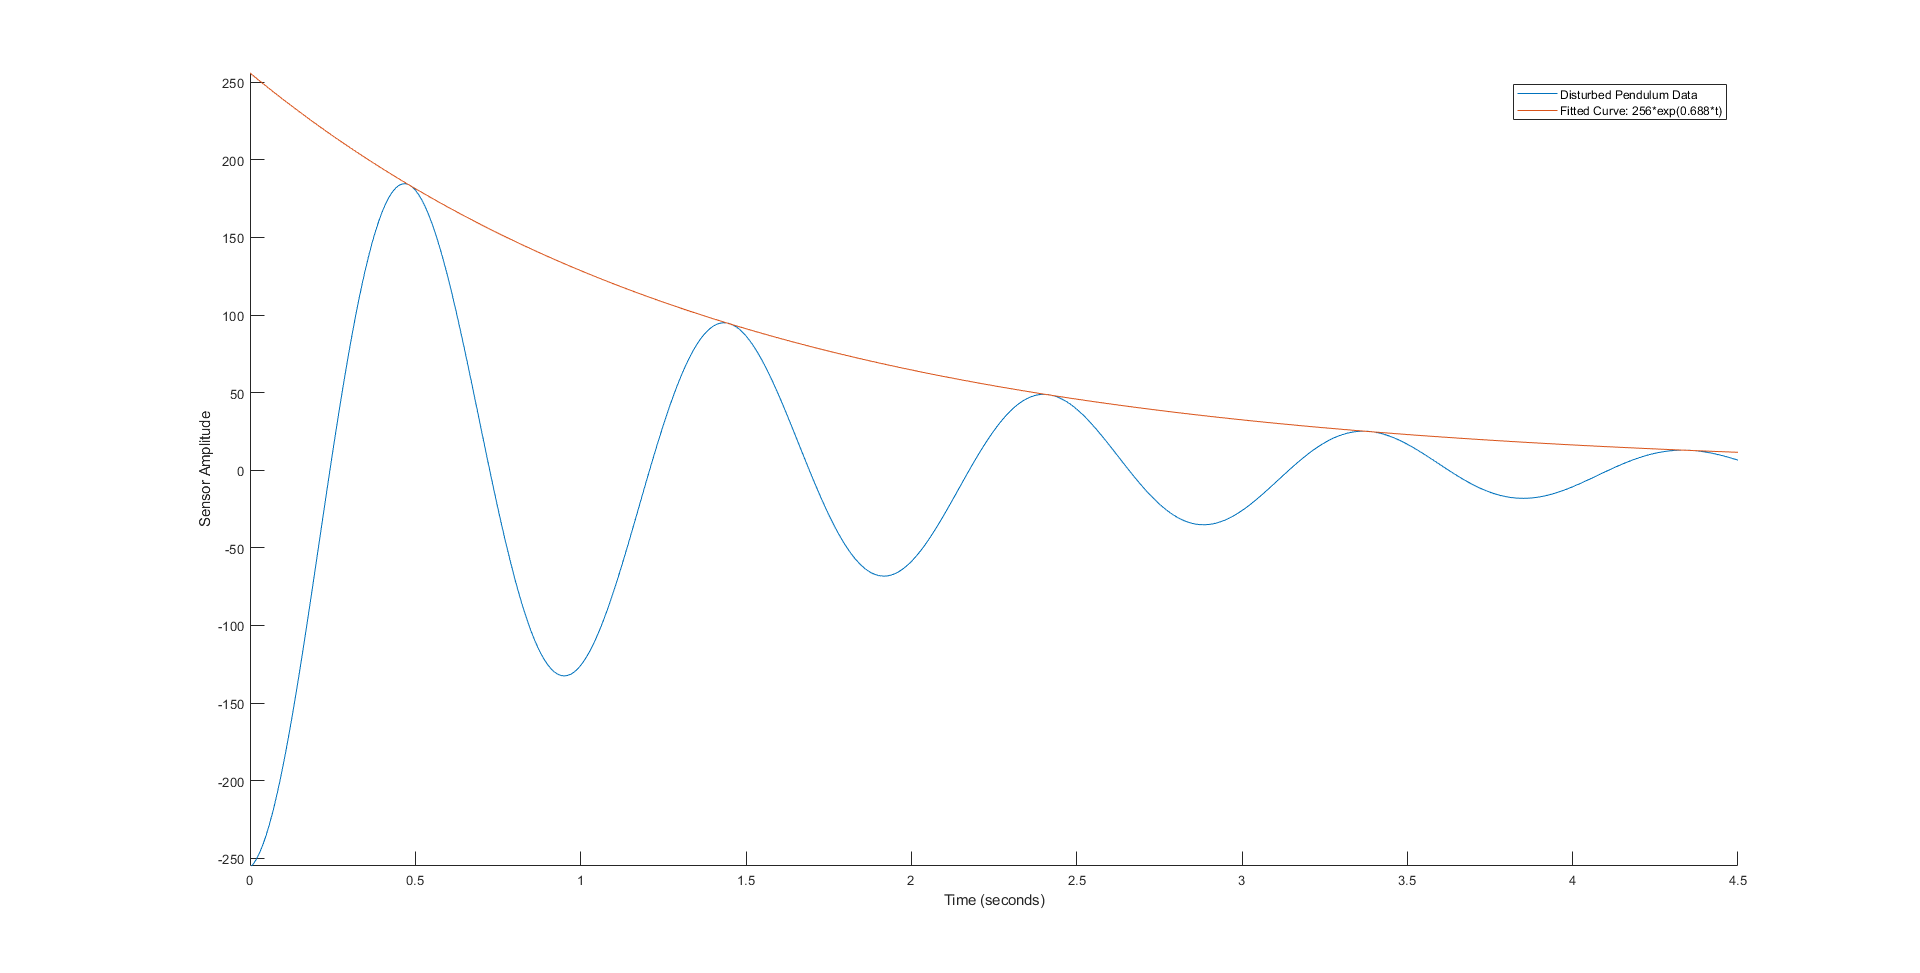
\includegraphics[width=\textwidth]{inc/fittedcurve.png}
        \caption{}
        \label{}
\end{figure}

\begin{figure}[h]
        \centering
        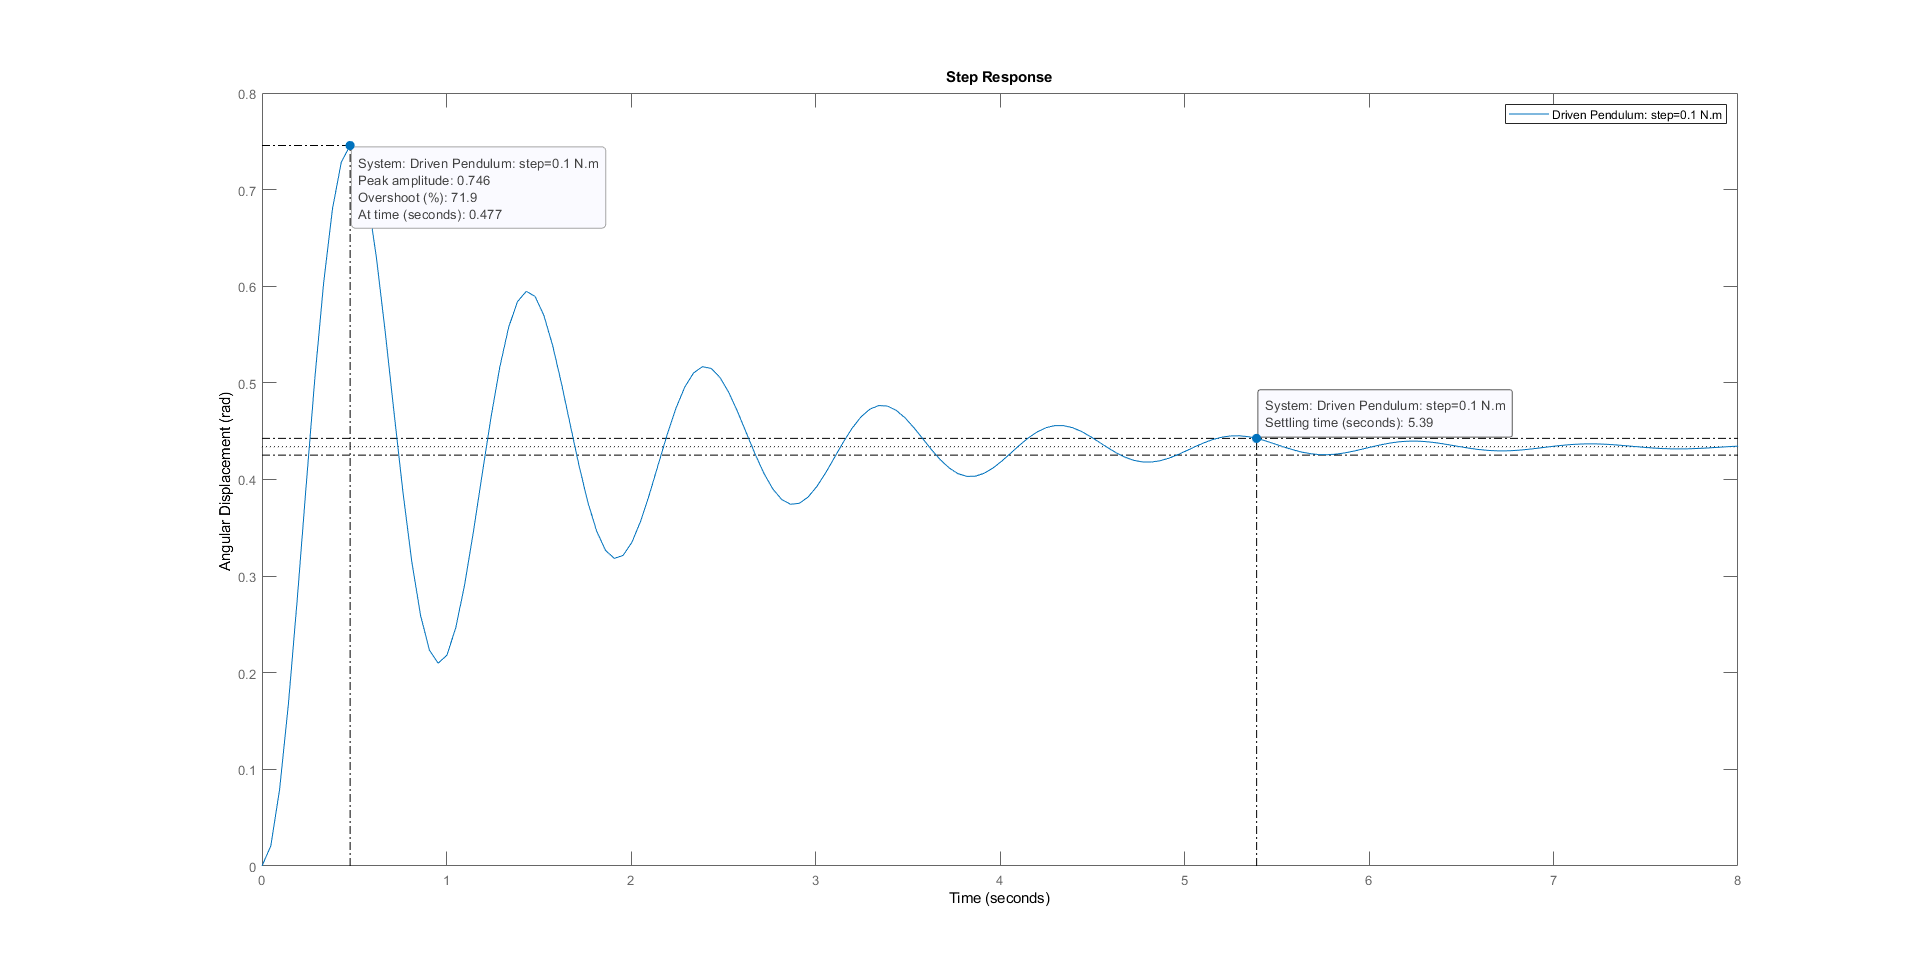
\includegraphics[width=\textwidth]{inc/pendulum.png}
        \caption{}
        \label{}
\end{figure}

\newpage
\subsection*{Full Open Loop TF}
\begin{figure}[h]
        \centering
        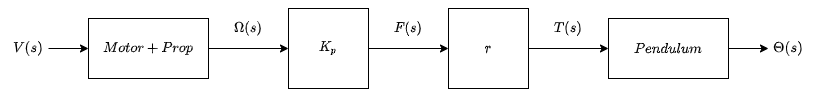
\includegraphics[width=0.75\textwidth]{inc/openloop_diagram.png}
        \caption{Block Diagram of DC Motor+Propeller System}
        \label{}
\end{figure}

\begin{align*}
        \frac{\Theta(s)}{V(s)} &= \frac{\frac{K_t}{L_aJ_m}}{s^2 + \frac{R_{a}J_{m} + L_{a}D_{m}}{L_{a}J_{m}}s + \frac{R_aD_m + K_tK_b}{L_aJ_m}} \cdot K_{p} \cdot r \cdot \frac{\frac{1}{J_{p}}}{s^{2} + \frac{c}{J_{p}}s + \frac{mgd}{J_{p}}} \\
        &= \frac{\frac{K_tK_pr}{J_pL_aJ_m}}{(s^2+\frac{c}{J_p}s+\frac{mgd}{J_p})(s^2+\frac{R_aJ_m+L_aD_m}{L_aJ_m}s+\frac{R_aD_m+K_tK_b}{L_aJ_m})}
\end{align*}



\begin{figure}[h]
        \centering
        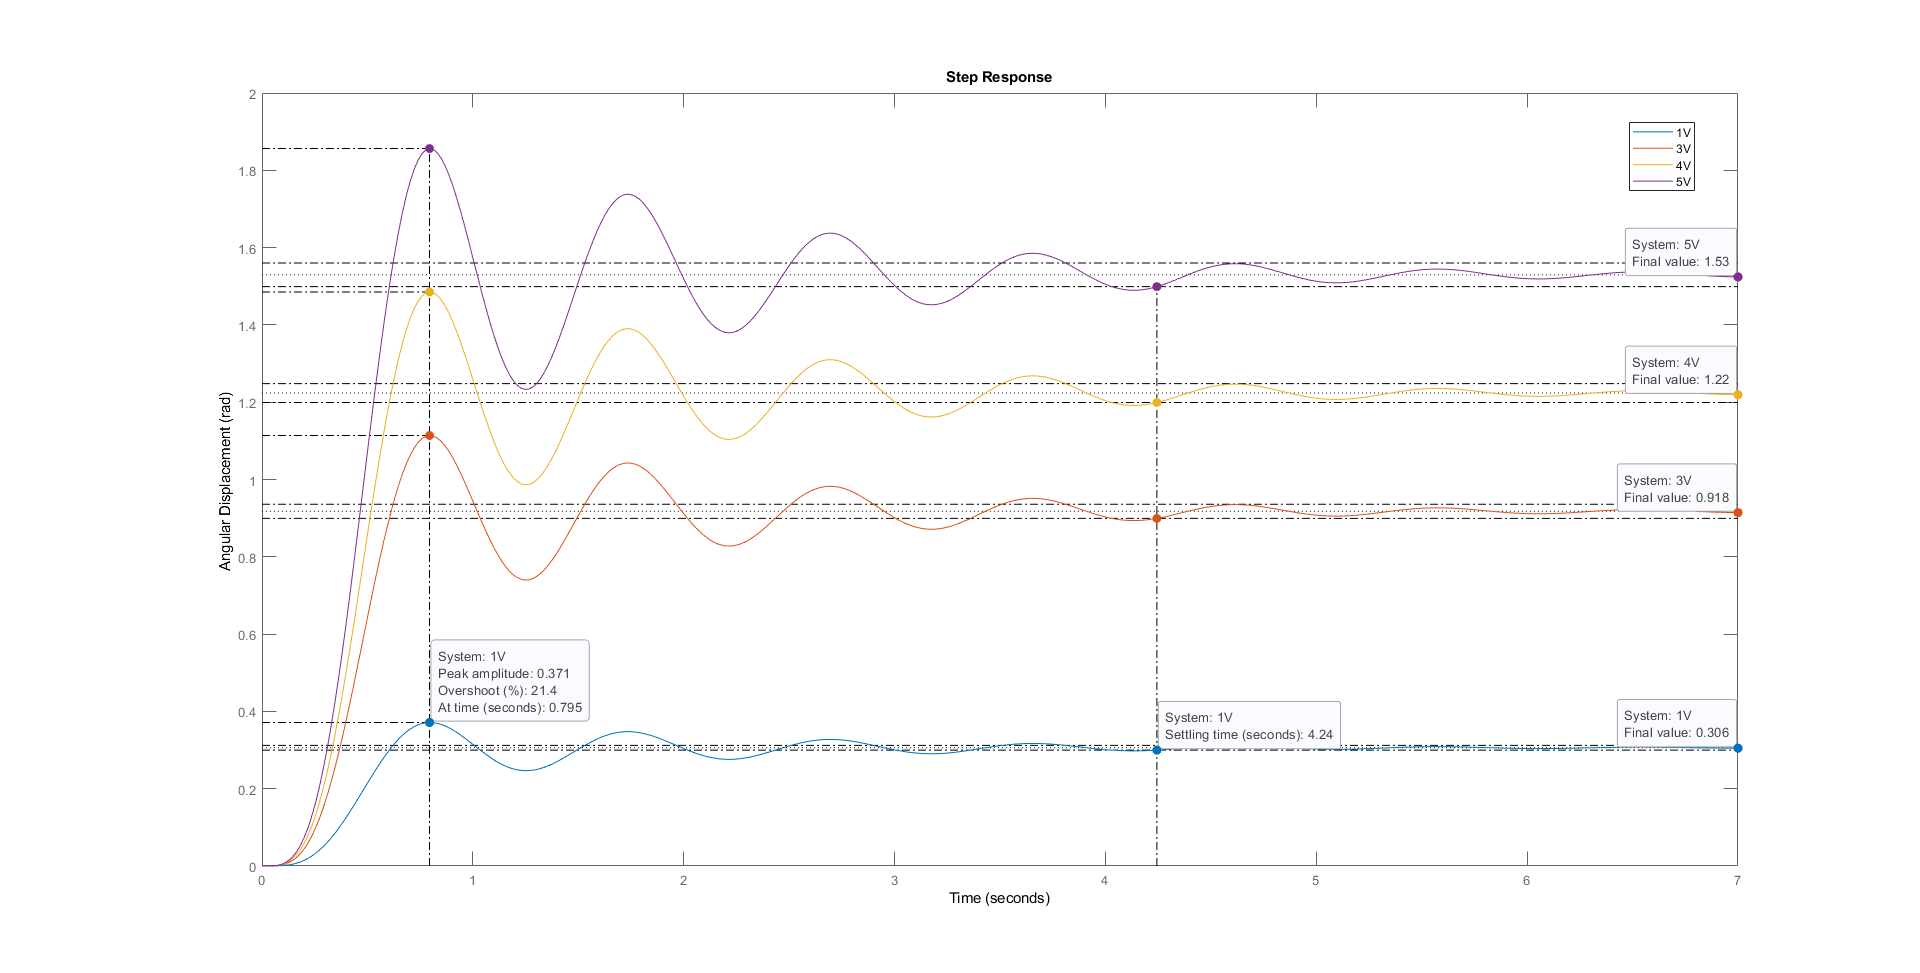
\includegraphics[width=\textwidth]{inc/combined_sys.png}
        \caption{}
        \label{}
\end{figure}

\newpage
\section{Discussion}
Big picture considerations, e.g. is your model useful or not?
\newpage
\section{Conclusions}

\nocite{*}
\bibliography{ref}
\bibliographystyle{IEEEtran}

\newpage

    \section{Full MatLab Code}
    \lstinputlisting{open_loop.m}
    \section{Lab Safety}
    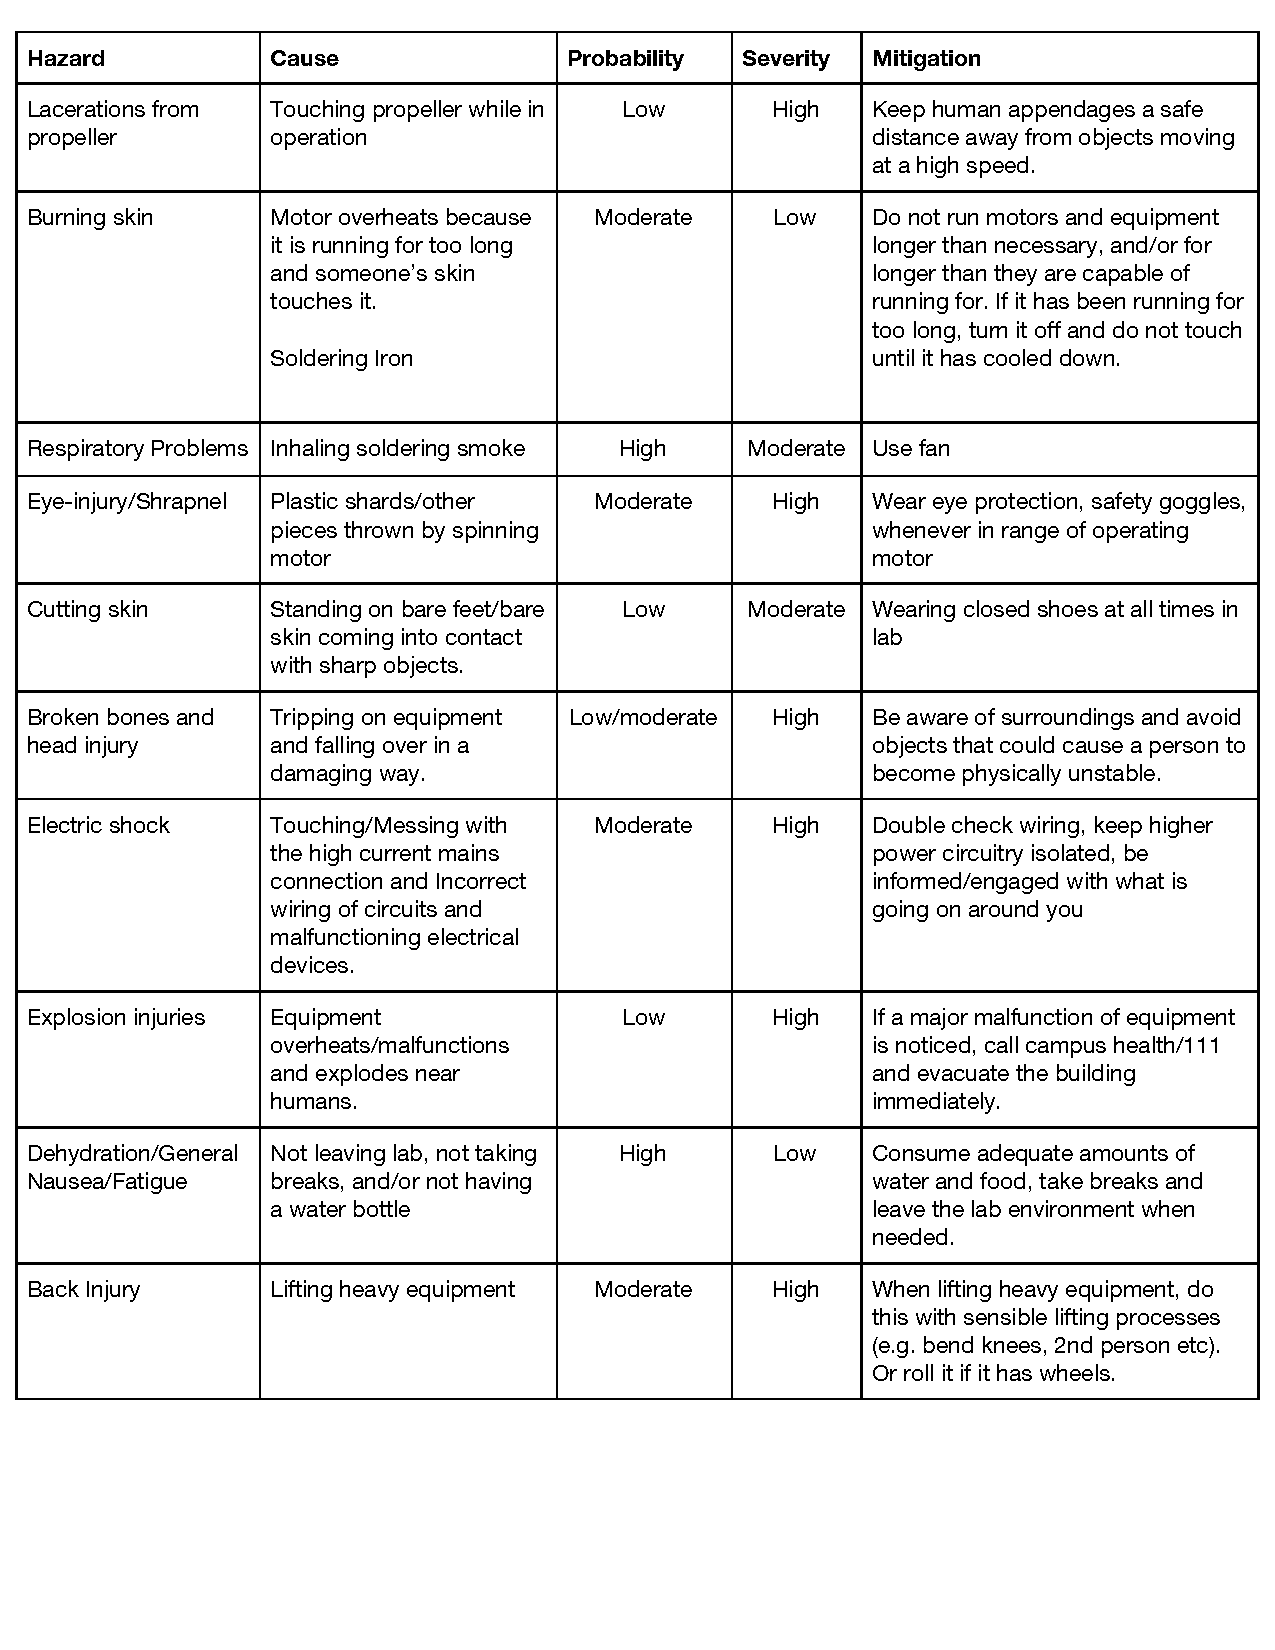
\includegraphics[width=\textwidth]{inc/safety.pdf}
    
\end{document}
